
    \documentclass{standalone}
\usepackage{tkz-fct}
\usepackage{tkz-euclide}
\usepackage{color}
\renewcommand*\familydefault{\sfdefault}
\usepackage{sansmath}
\sansmath
\definecolor{gray75}{gray}{0.75}
\begin{document}
 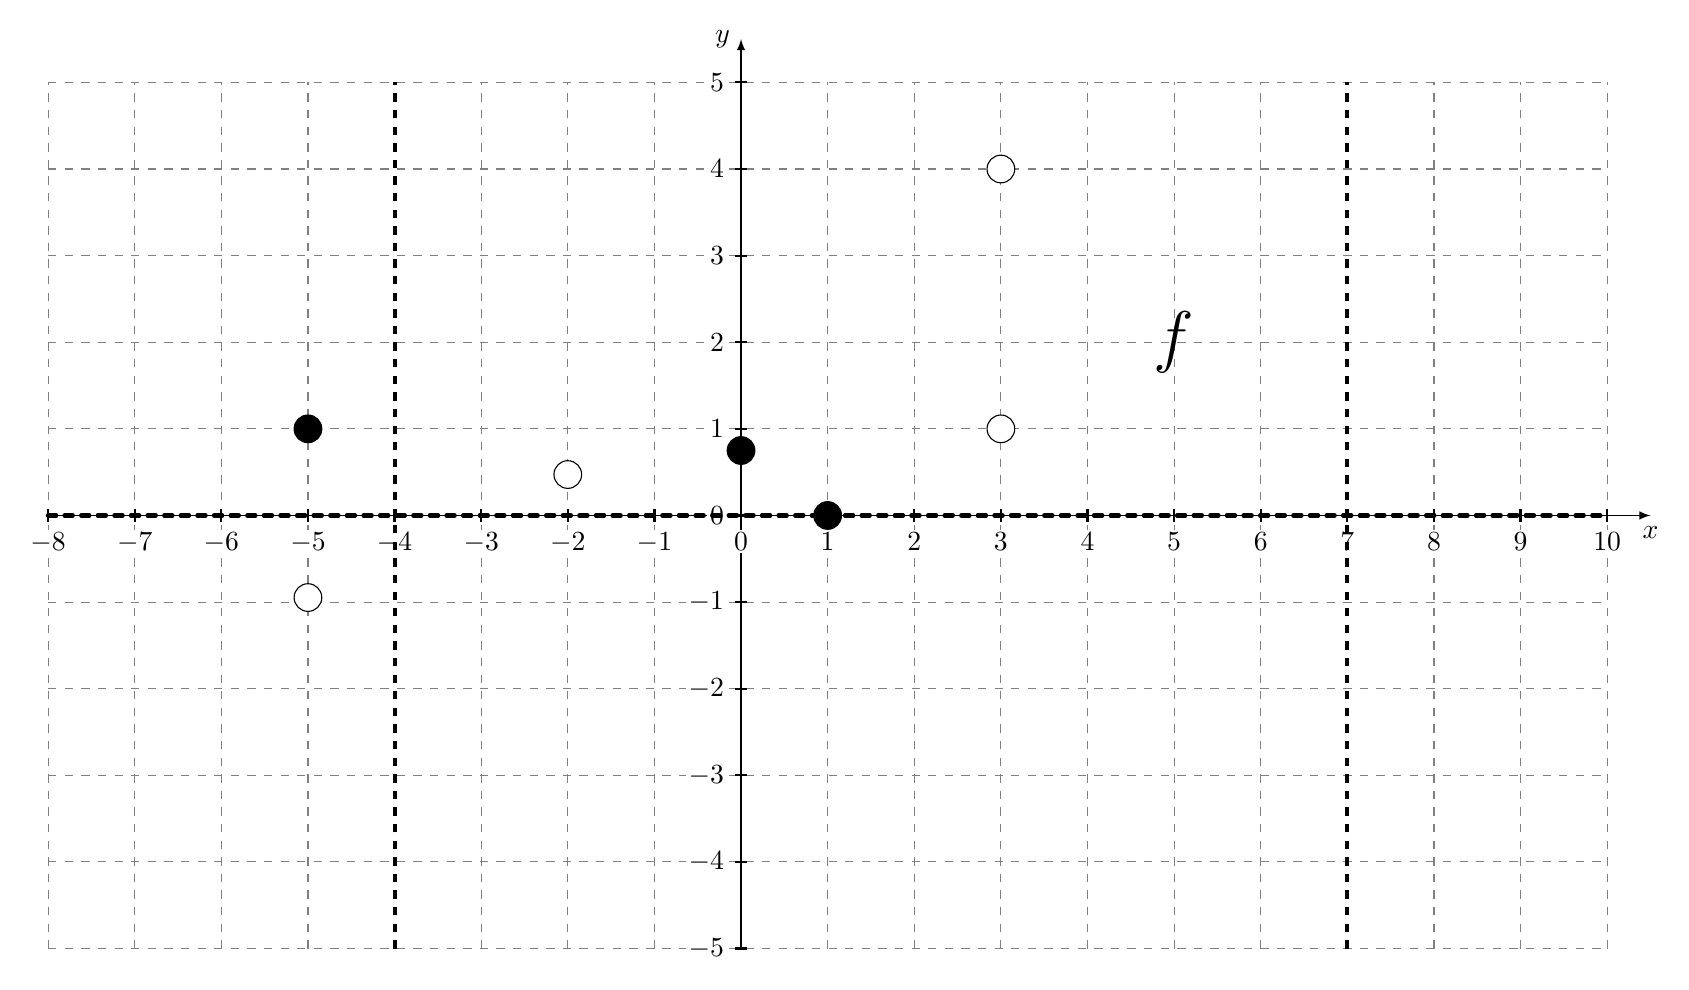
\begin{tikzpicture}[scale=1.1]
   \tkzInit[xmax=10.0,ymax=5.0,xmin=-8.0 ,ymin=-5.0]
   \begin{scope}[dashed]
     \tkzGrid
   \end{scope}
   \tkzDrawX[label={$x$}]
   \tkzDrawY[label={$y$}]
   \tkzLabelX
   \tkzLabelY
   \tkzFctPar[line width=2pt,samples=400,domain=0:1]{((440226863575466*t**3 - 1979382675538911*t**2 + 2639722970902110*t - 2251799813685248)/281474976710656)}{(-(286789224270953127*t**3 + 386976094683223935*t**2 + 43207741723205901*t + 3602879701896397)/144115188075855872)}
\tkzFctPar[line width=2pt,samples=400,domain=0:1]{((t - 1)*(880453727150932*t**2 + 2197249963198723*t + 2201134317877330)/562949953421312)}{((20716558285904281*t**3 - 93224512286567577*t**2 + 124299349715424000*t - 45035996273704960)/9007199254740992)}
\tkzFctPar[line width=2pt,samples=400,domain=0:1]{((3602879701896395*t**3 - 5404319552844594*t**2 + 10808639105689191*t + 4503599627370496)/4503599627370496)}{(t**2*(1801439850948199*t + 2702159776422297)/1125899906842624)}
\tkzFctPar[line width=2pt,samples=400,domain=0:1]{((880453727150932*t**3 - 3957988532514561*t**2 + 5278669123240959*t + 1688849860263936)/562949953421312)}{(-(675539944105575*t**3 + 1013309916158361*t**2 - 281474976710656)/281474976710656)}

   
                \tkzDefPoint(-8.0,0.0){A}

                \tkzDefPoint(10.0,0.0){B}

                \tkzDrawSegment[style=dashed,line width = 1.5pt](A,B)

                \tkzVLine[style=dashed,line width = 1.5pt]{-4.0}
\tkzVLine[style=dashed,line width = 1.5pt]{-4.0}
\tkzVLine[style=dashed,line width = 1.5pt]{7.0}

   \tkzDrawPoint[size=10,color=black,fill=black](-5.0,1.0)
\tkzDrawPoint[size=10,color=black,fill=black](0.0,0.75)
\tkzDrawPoint[size=10,color=black,fill=black](1.0,0.0)
\tkzDrawPoint[size=10,color=black,fill=white](3.0,4.0)
\tkzDrawPoint[size=10,color=black,fill=white](3.0,1.0)
\tkzDrawPoint[size=10,color=black,fill=white](-5.000000000000001,-0.9476816589440207)
\tkzDrawPoint[size=10,color=black,fill=white](-2.0,0.4726791342321024)


   \tkzText(5,2){\Huge$f$}

\end{tikzpicture}
\end{document}

    